\documentclass{article}

\usepackage[utf8]{inputenc}
\usepackage{scrextend}
\usepackage{graphicx}
\usepackage[edges]{forest}

\definecolor{foldercolor}{RGB}{124,166,198}

\tikzset{pics/folder/.style={code={%
    \node[inner sep=0pt, minimum size=#1](-foldericon){};
    \node[folder style, inner sep=0pt, minimum width=0.3*#1, minimum height=0.3*#1, above right, xshift=0.05*#1] at (-foldericon.west){};
    \node[folder style, inner sep=0pt, minimum size=#1] at (-foldericon.center){};}
    },
    pics/folder/.default={20pt},
    folder style/.style={draw=foldercolor!80!black,top color=foldercolor!40,bottom color=foldercolor}
}

\forestset{is file/.style={edge path'/.expanded={%
        ([xshift=\forestregister{folder indent}]!u.parent anchor) |- (.child anchor)},
        inner sep=1pt},
    this folder size/.style={edge path'/.expanded={%
        ([xshift=\forestregister{folder indent}]!u.parent anchor) |- (.child anchor) pic[solid]{folder=0.7*#1}}, inner sep=0.2*#1},
    folder tree indent/.style={before computing xy={l=0.6*#1}},
    folder icons/.style={folder, this folder size=#1, folder tree indent=3*#1},
    folder icons/.default={12pt},
}
% Margins
\topmargin=-0.45in
\evensidemargin=0in
\oddsidemargin=0in
\textwidth=6.5in
\textheight=9.0in
\headsep=0.25in
\graphicspath{ {./} }

\title{Progetto di Automated Reasoning\\2021-2022}

\author{ Christian Londero }
\date{15 Febbraio 2022}

\begin{document}
\maketitle

\section{Definizione del problema}
Si consideri una scacchiera $n$ x $n$ ($n$ è dato in input). Si hanno a disposizione $l$ pezzi a forma di L, $s$ pezzi a forma di quadrato e $r$ pezzi a forma di rettangolo (si veda la figura, la dimensione del rettangolo è 3 x 1, il quadrato è 2 x 2 e il lato lungo della L è 2). $l$, $s$, $r$ sono dati in input. L'obbiettivo è di riempire la scacchiera con i pezzi a disposizione in maniera tale da minimizzare le celle vuote/free. Il requisito aggiuntivo è che $f$ celle (date in input) siano già occupate (quindi vietate).\\
Si veda l'esempio (le celle grigie sono già occupate/vietate).

\subsection{Considerazioni}
Si presenterà un algoritmo che tenta di minimizzare le celle empty scegliendo da un sottoinsieme dei pezzi. \\
Quindi si può dare in input un numero molto alto di pezzi al fine di "semplificare" la minimizzazione, sebbene si rischia in questo caso di fare utilizzare gli stessi tipi di pezzi quasi ovunque.\\
Nella sezione dei risultati vedremo infatti che se abbiamo a disposizione un elevato numero di pezzi ($3*l + 4*s + 3*r \gg n*n$) allora il solving è "facile", rispetto a un numero quasi giusto di pezzi ($3*l + 4*s + 3*r \simeq n*n$).

\section{Struttura della folder}
\begin{forest}
    for tree={font=\sffamily, grow'=0,
    folder indent=.9em, folder icons,
    edge=densely dotted}
    [main folder
      [images
          [wallpapers]
          [logo.pdf, is file]]
      [tex-files
          [chapter1.tex, is file]]
      [main.tex, is file]
      [main.aux, is file]
    ]
  \end{forest}
\section{Soluzione}
L'idea utilizzata per la realizzazione dei modelli è la stessa sia per il modello in minizinc che per quello in asp. Parlando a livello non-implementativo, è la seguente: il programma prende in input i seguenti parametri:
\begin{itemize}
    \item \texttt{n} (intero): dimensione della board;
    \item \texttt{l} (intero): numero di L (2x2) disponibili;
    \item \texttt{s} (intero): numero di quadrati (2x2) disponibili;
    \item \texttt{r} (intero): numero di rettangoli (1x3) disponibili;
    \item \texttt{f} (intero): numero di celle vietate/forbidden/già occupate;
    \item \texttt{forbidden} (array): array lungo $f$ di coordinate $X,Y$ (sono dei fatti/facts in asp ovviamente).
\end{itemize}
La board è una matrice (array bi-dimensionale) $n$ x $n$ il cui dominio è definito dalla seguente enumerazione: \texttt{XXX, EEE, S11, S12, S13, S14, R11, R12, R13, R21, R22, R23, L11, L12, L13, L21, L22, L23, L31, L32, L33, L41, L42, L43}.\\
Al fine di rendere comprensibile l'enumerazione si osservi la figura qui di seguito.\\
\begin{figure}[ht!]
    \centering
    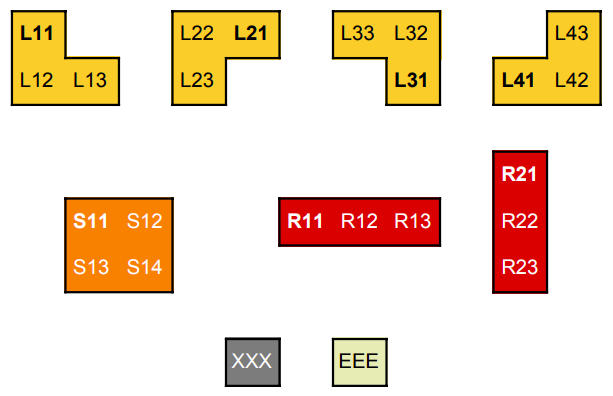
\includegraphics[width=0.7\textwidth]{shapes}
    \caption{Tutte le possibili shapes con rotazioni}
\end{figure}
Quindi ogni cella può assumere uno di quei valori dell'enumerazione, si è quindi proceduto a definire dei vincoli che mantengano le forme corrette.\\
Ho utilizzato tale "metodo" al fine di evitare sovrapposizioni indesiderate dei pezzi. \\

\subsection{Ulteriori idee}
Avevo pensato ad altre due modellazioni che però nell'implementazione poi si sono rivelate errate/inefficienti:
\begin{itemize}
    \item indicare con 1 le L, con 2 i quadrati e con 3 i rettangoli, con 0 le empty cells e con -1 i forbidden; tuttavia, sebbene il dominio in questo casi sia notevolmente ridotto, con tale metodo non si riescono a gestire efficientemente le sovrapposizioni di forme uguali con diverse rotazioni
    \item enumerare ogni pezzo mantenendo il tipo salvato in un "array" lungo $k$ con $k=l+s+r$ (per esempio, ignorando le celle empty e forbidden, se abbiamo $k=2+1+3$ avremmo che il dominio delle celle della board è $1..k$ = $1..6$ e manteniamo un ulteriore array lungo k per indicare il tipo: [1,1,2,3,3,3]), in modo tale che il tipo indichi quali constraint il pezzo i-esimo debba avere e non ci sono sicuramente sovrapposizioni in quanto un pezzo di forma uguale avrebbe un $j!=i$ come "valore" e ogni "valore" può comparire al più 3 o 4 volte nella board a seconda della forma (rispettivamente se L/rettangolo o quadrato); tuttavia questo metodo si è rivelato altamente inefficiente in quanto i domini erano molto più grandi rispetto alla soluzione scelta e portavano quindi a tempi molto più elevati anche con strategie di \texttt{int\_search} (per minizinc) personalizzate;
\end{itemize}

\section{Risultati minizinc}


\end{document}